\documentclass{book}

\usepackage[english, bulgarian]{babel}
\selectlanguage{bulgarian}

\usepackage[pdftex, bookmarks, linktocpage]{hyperref}

\usepackage[pdftex]{graphicx}
\graphicspath{{images/}}

\usepackage{xcolor}
\definecolor{lightgray}{gray}{0.95}

\usepackage{listings}
\lstset{backgroundcolor=\color{lightgray}}
\renewcommand{\lstlistingname}{Листинг}
\renewcommand{\lstlistlistingname}{Списък на листингите}

\title{Оформление на научни документи с LaTeX}
\author{Тодор Балабанов, Красимира Стоянова-Чокова}
\date{\today}

\begin{document}

\maketitle

\frontmatter

\tableofcontents
\listoffigures
\lstlistoflistings
%\listoftables

\mainmatter

\chapter*{Предговор}
LaTeX е безплатен софтуер с отворен код за оформяне на документи. LaTeX не е текстообработваща програма, а е език за тагиране на документи.

Първоначално е създадено от Leslie Lamport и е базиран на машината за набор TeX, създадена от Donald Knuth. Често го се ползва названието TeX, което също означава LaTeX.

LaTeX е много добър избор за създаване и поддържане на документи в областта на науката или за техническа документация. Едно от най-силните предимства на LaTeX е възможността за представяне на математически формули. За студенти и учени, LaTeX е способен да произведе документи с много високо качество, като гарантира стабилност на крайния резултат.

Друга много силна страна на системата е възможността за създаване на референции, като таблици на съдържанието, фигурите, таблиците, листингите и други, в съчетание с възможности за автоматично номериране, изграждане на библиография и индекс на използваните думи.

Осен полезността за хора занимаващи се с наука LaTeX дава и много голяма степен на гъвкавост. Съществуват множество шаблони за книги, писма, циркулярни писма, презентации, музикален нотопис и много други. Отвореният характер на системата е позволила на стотици потребители да създадат хиляди шаблони, стилове и полезни инструменти. Всеки един от вас може да се присъедини в разширяването на възможностите, предоставени от тази система.

Фундаментална концепция в LaTeX е разделението между съдържание и оформление. Авторът не е толкова ангажиран в оформлението и може значително по-сериозно да се концентрира върху създаването на съдържание. В други системи за текстова обработка, авторите са много по-ангажирани с паралелно оформление на своето съдържание. При LaTeX този процес се управлява през тагове (команди), които бързо се научават от създателите на LaTeX документи. Чрез промяна на класовете документи и пакетите, бързо и лесно може да се променя цялостното оформление на документа.

Тъй като LaTeX е софтуер с отворен код, то този инструмент е достъпен за почти всякакви операционни системи, най-основните сред които са Windows, MacOS и Linux. Основните файлови формати, ползвани в LaTeX, са текстови, така че могат да се четат и редактират под всякакви операционни системи. Това позволява LaTeX да създаде почти идентични резултатни документи в различните операционни системи. Системата TeX има множество различни дистрибуции, но в това изложение ще се ползва MiKTeX в комбинация с Texmaker, под операционна система Windows. 

За да се поддържа високата преносимост на LaTeX между различните операционни системи, не се използва графичен потребителски интерфейс. Авторите могат да създават своите документи с всеки текстов редактор, който предпочитат. Има създадени множество текстови редактори, специално предназначени за TeX документи. Такъв редактор е Texmaker, който се поддържа на Windows, MacOS и Linux. Това го прави изключително подходящ за целите на настоящото изложение. Веднъж свикнал потребителят с интерфейса на Texmaker, под някоя от операционните системи, то ползването му под другите операционни системи е почти идентично. 

Основните резултатни документи, които LaTeX генерира са в PDF формат. Това прави резултатните документи изключително преносими и използваеми под всякакви операционни системи и хардуер. PDF е формат, който изглежда идентично на различните платформи и го прави универсален за обмен на информация. Също така, резултатните документи могат да са и в други файлови формати, като HTML, DVI, PostScipt, ePub и други. Всичко това позволява информацията да се представя както за печатно издаване, така и за онлайн съдържание.

Голямо предимство в LaTeX е, че изходните текстове не се съдържат в комерсиален файлов формат или във файлови формати, които имат склонността да се превръщат в морално остарели и за които се налага използването на специално създадени конвертори. Не на последно място, намалява се рискът от заразяване с вируси, нещо което е възможно във файловите формати на други софтуери за текстообработка.




\part{Базови познания}

\chapter{Първи стъпки}
За работа с LaTeX има два основни начина - на локалната машина и в облачна услуга. Най-популярната облачна услуга е Overleaf, като тя дава множество възможности и е изключително лесна за усвояване, ако потребителят вече има опит с някоя от локалните инсталации на LaTeX системата. В настоящето изложение ще бъде представена интегрираната среда за създаване на документи Texmaker, в комбинация с MiKTeX, под операционна система Microsoft Windows.

\section{Инсталиране на MiKTeX}

MiKTeX е дистрибуция на TeX/LaTeX системата, работеща под операционна система Windows. Предоставя изчерпателен набор от инструменти и пакети за създаване и форматиране на документи, особено в академични и научни области. MiKTeX включва необходимите програми, шрифтове и макроси за ефективна работа с TeX/LaTeX на операционна система Windows. Той опростява процеса на инсталиране и гарантира, че потребителите ще имат достъп до различни пакети и ресурси за подготовка на документи.

Инсталирането на MiKTeX започва със сваляне на инсталационния файл от официалният сайт на продукта (Фиг. \ref{figure-0001}).

\begin{figure}
  \centering
  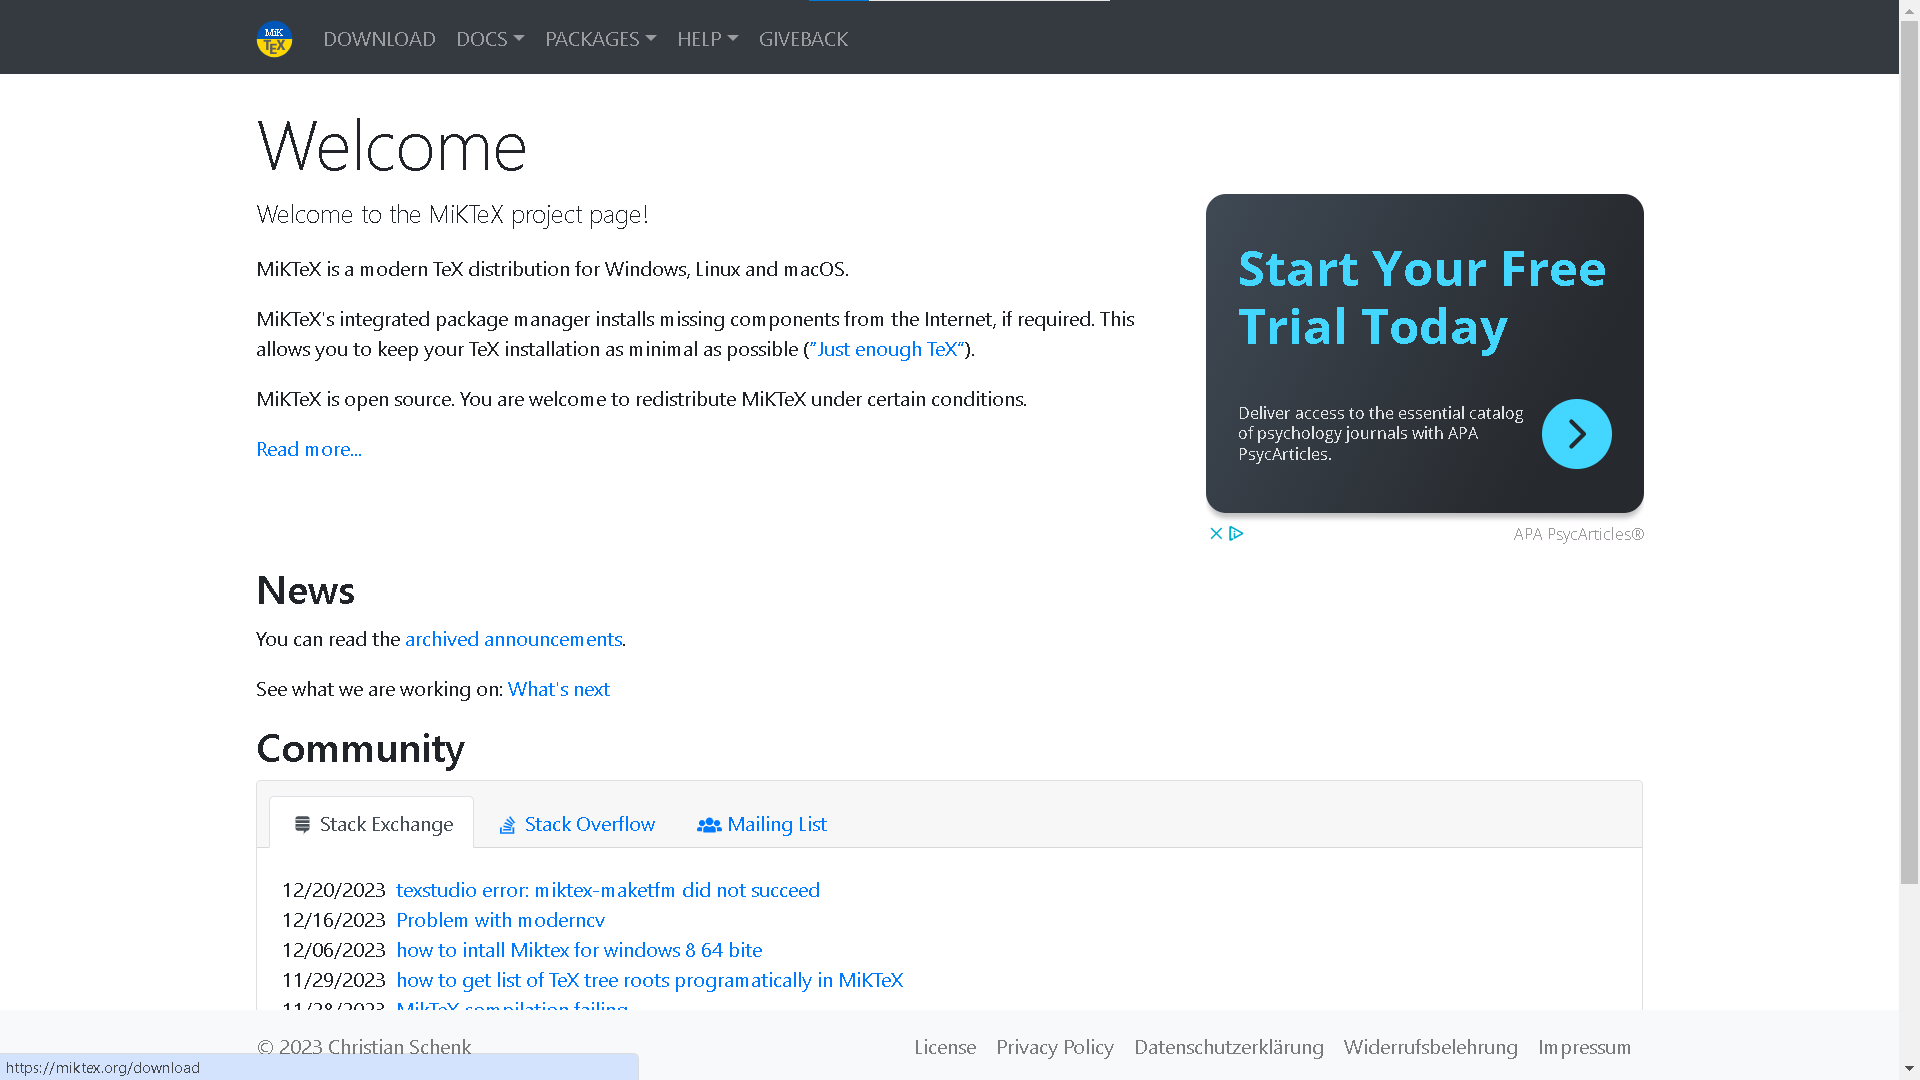
\includegraphics[width=1.0\linewidth,height=0.5\linewidth]{figure-0001.png}
  \caption{Начална уеб страница на MiKTeX}
\label{figure-0001}
\end{figure}

MiKTeX е достъпен за няколко различни операционни системи, но за нуждите на текущото изложение се използва версията на Windows (Фиг. \ref{figure-0002}).

\begin{figure}
  \centering
  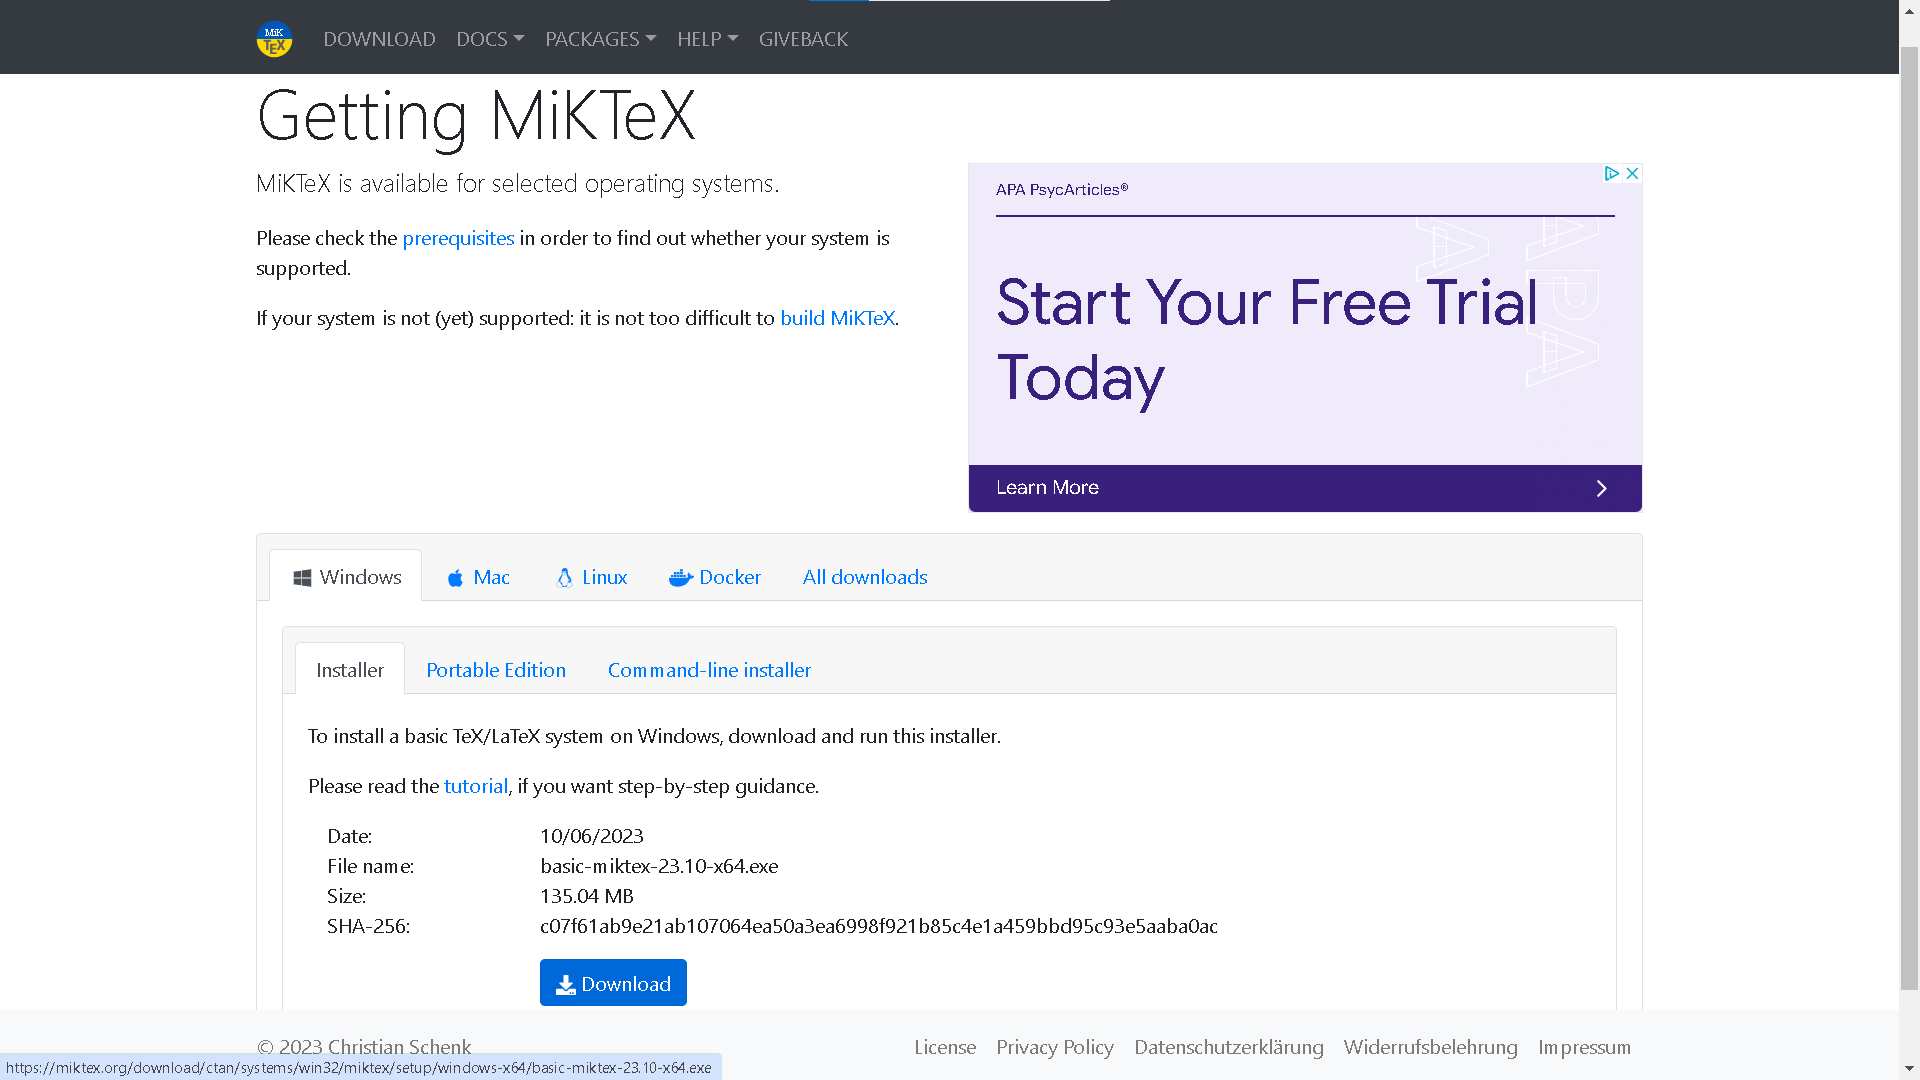
\includegraphics[width=1.0\linewidth,height=0.5\linewidth]{figure-0002.png}
  \caption{Избор на инсталационен файл за MiKTeX}
\label{figure-0002}
\end{figure}

Както всеки друг сериозен софтуерен продукт и MiKTeX е съпроводен с обши условия за ползване. Потребителят трябва да се съгласи с тях (Фиг. \ref{figure-0003}) веднага след като стартира изпълнимият файл на инсталатора.

\begin{figure}
  \centering
  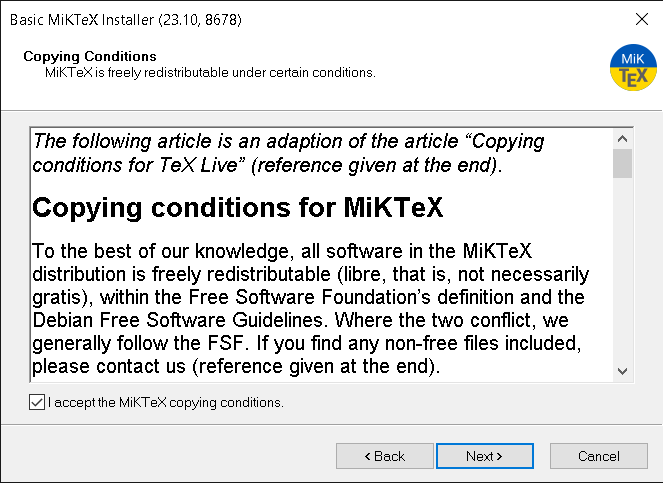
\includegraphics[width=1.0\linewidth,height=0.5\linewidth]{figure-0003.png}
  \caption{Диалогов прозорец за съгласие с условията за ползване на MiKTeX}
\label{figure-0003}
\end{figure}

Както при повечето съвременни операционни системи и в Windows се дава възможност за избор дали програмата да бъде инсталирана за конкретния потребители на системата (Фиг. \ref{figure-0004}) или за всички потребители.

\begin{figure}
  \centering
  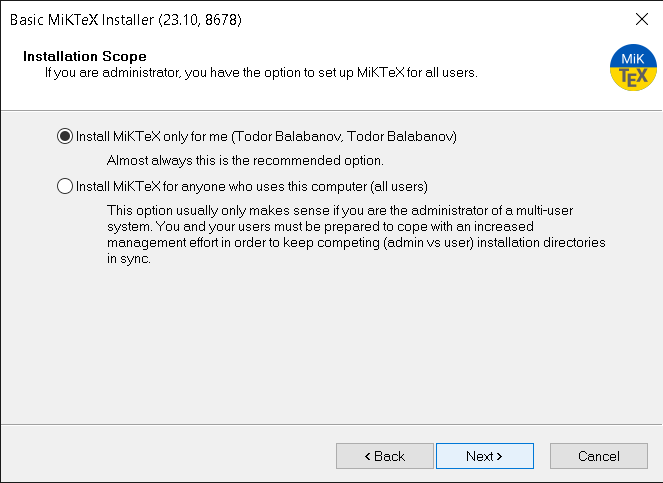
\includegraphics[width=1.0\linewidth,height=0.5\linewidth]{figure-0004.png}
  \caption{Избор на потребители с достъп до MiKTeX}
\label{figure-0004}
\end{figure}

За разлика от операционните системи, които под една или друга форма произлизат от операционната система Unix, в Windows потребителят сам трябва да посочи инсталационната директория (Фиг. \ref{figure-0005}) на софтуера, който той сам инсталира.

\begin{figure}
  \centering
  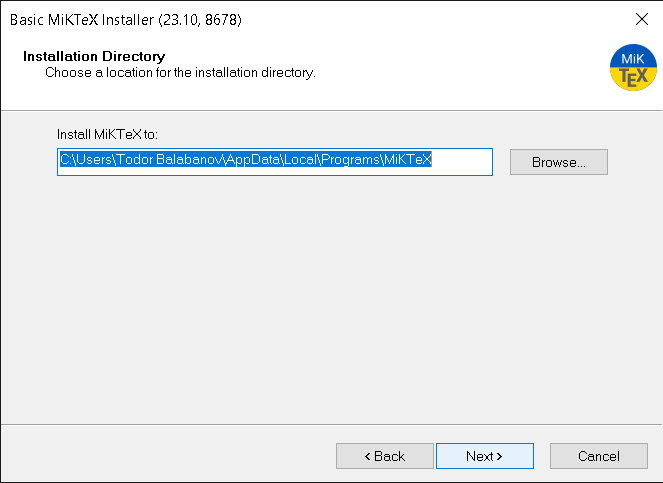
\includegraphics[width=1.0\linewidth,height=0.5\linewidth]{figure-0005.png}
  \caption{Инсталационна директория на MiKTeX}
\label{figure-0005}
\end{figure}

Тъй като LaTeX е система организирана на модулен принцип, към ядрото на системата могат да се инсталират допълнителни пакети. Не е нужно, а и би направило твърде тромава цялата система, ако всички налични пакети бъдат инсталирани предварително. Поради тези причини, допълнителните пакети се инсталират при първа поява за тяхната необходимост. При инсталирането на MiKTeX потребителят трябва да избере политиката за инсталиране на пакети. За да има контрол върху това, което бива инсталирано, то най-удачният избор е, при нужда от пакет, потребителят първо да бъде попитан (Фиг. \ref{figure-0006}).

\begin{figure}
  \centering
  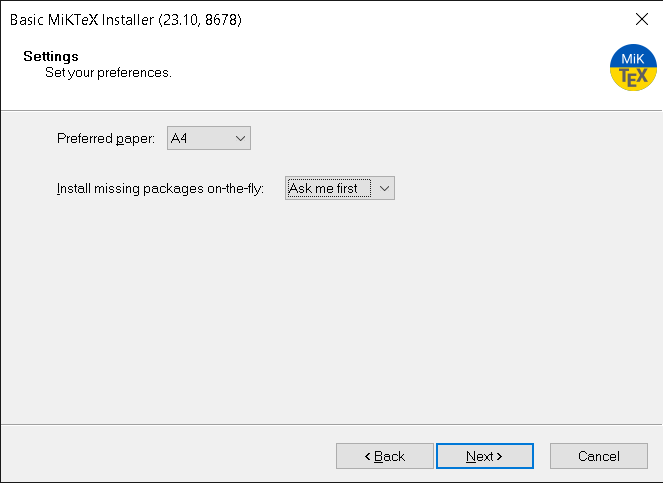
\includegraphics[width=1.0\linewidth,height=0.5\linewidth]{figure-0006.png}
  \caption{Избор на политика за инсталиране на пакети}
\label{figure-0006}
\end{figure}

След установяване на първоначалните параметри за изпълнение на инсталацията, процесът по инсталиране може да бъде стартиран (Фиг. \ref{figure-0007}).

\begin{figure}
  \centering
  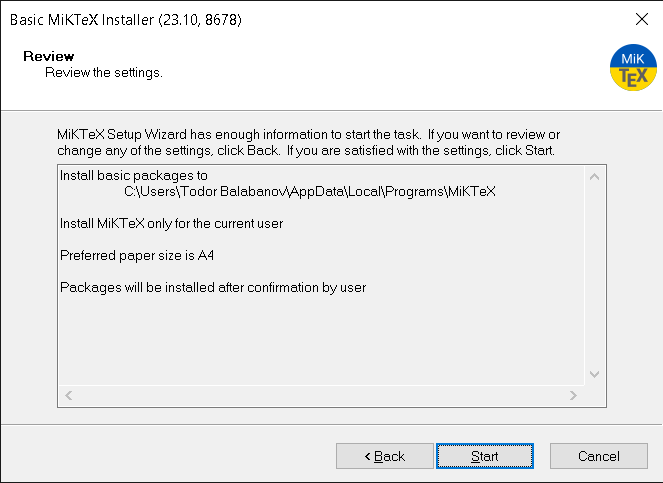
\includegraphics[width=1.0\linewidth,height=0.5\linewidth]{figure-0007.png}
  \caption{Стартиране на процеса по инсталация на MiKTeX}
\label{figure-0007}
\end{figure}

Чрез два прогрес бара, програмата за инсталиране на MiKTeX отразява напредъка в осъществяването на процеса (Фиг. \ref{figure-0008}).

\begin{figure}
  \centering
  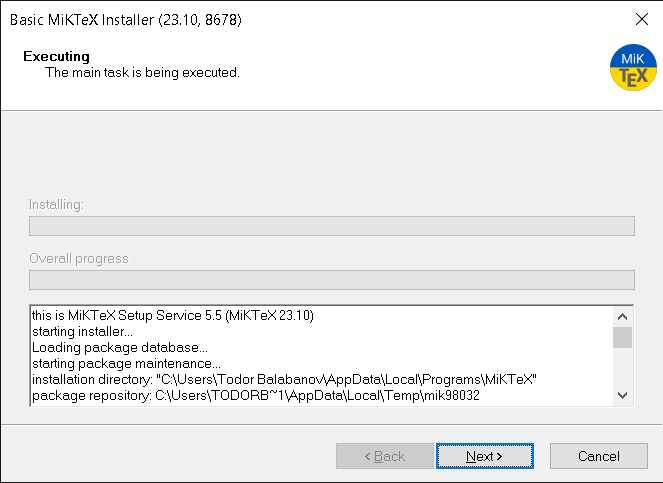
\includegraphics[width=1.0\linewidth,height=0.5\linewidth]{figure-0008.png}
  \caption{Прогрес на процедурата по инсталация}
\label{figure-0008}
\end{figure}

След инсталирането на основната част от продукта, потребителят има възможност да извърши проверка за наличие на нови версии (Фиг. \ref{figure-0009}).

\begin{figure}
  \centering
  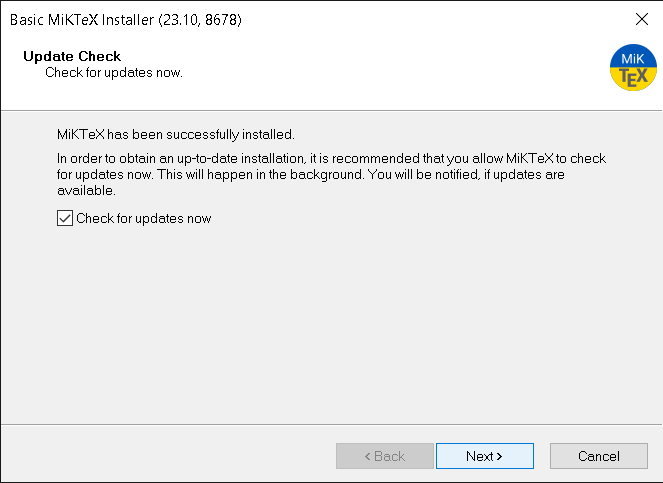
\includegraphics[width=1.0\linewidth,height=0.5\linewidth]{figure-0009.png}
  \caption{Избор за проверка на нови версии}
\label{figure-0009}
\end{figure}

Процедурата по инсталиране приключва със съобщение за начина по който е завършил процесът и с възможност за препращане към прозорец с допълнителна информация (Фиг. \ref{figure-0010}).

\begin{figure}
  \centering
  
\includegraphics[width=1.0\linewidth,height=0.5\linewidth]{figure-0010.png}
  \caption{Диалогов прозорец с информация за извършеното инсталиране}
\label{figure-0010}
\end{figure}

MiKTeX осигурява основната функционалност за създаването на TeX документи, но за по-комфортна работа е разумно да се инсталира и специализиран текстов редактор.

\section{Инсталиране на Texmaker}

Texmaker е безплатен, многоплатформен LaTeX редактор, който предоставя интегрирана среда за разработка за работа със системата за набор на документи LaTeX. Той предлага удобен за потребителя интерфейс с функции като подчертаване на синтаксис, допълване на код, проверка на правописа и вграден PDF преглед за оформление на документи. Texmaker позволява на потребителите да създават и управляват LaTeX документи ефективно, като предлага инструменти за бърза навигация през големи документи, управление на множество файлове едновременно и компилиране на LaTeX код за генериране на PDF изход. Texmaker е предпочитан избор сред потребителите на LaTeX поради своята лекота на използване, гъвкавост и изчерпателен набор от функции за писане и редактиране на документи.

Както при MiKTeX, инсталирането на Texmaker започва със сваляне на инсталационния файл от официалният сайт на продукта (Фиг. \ref{figure-0011}).

\begin{figure}
  \centering
  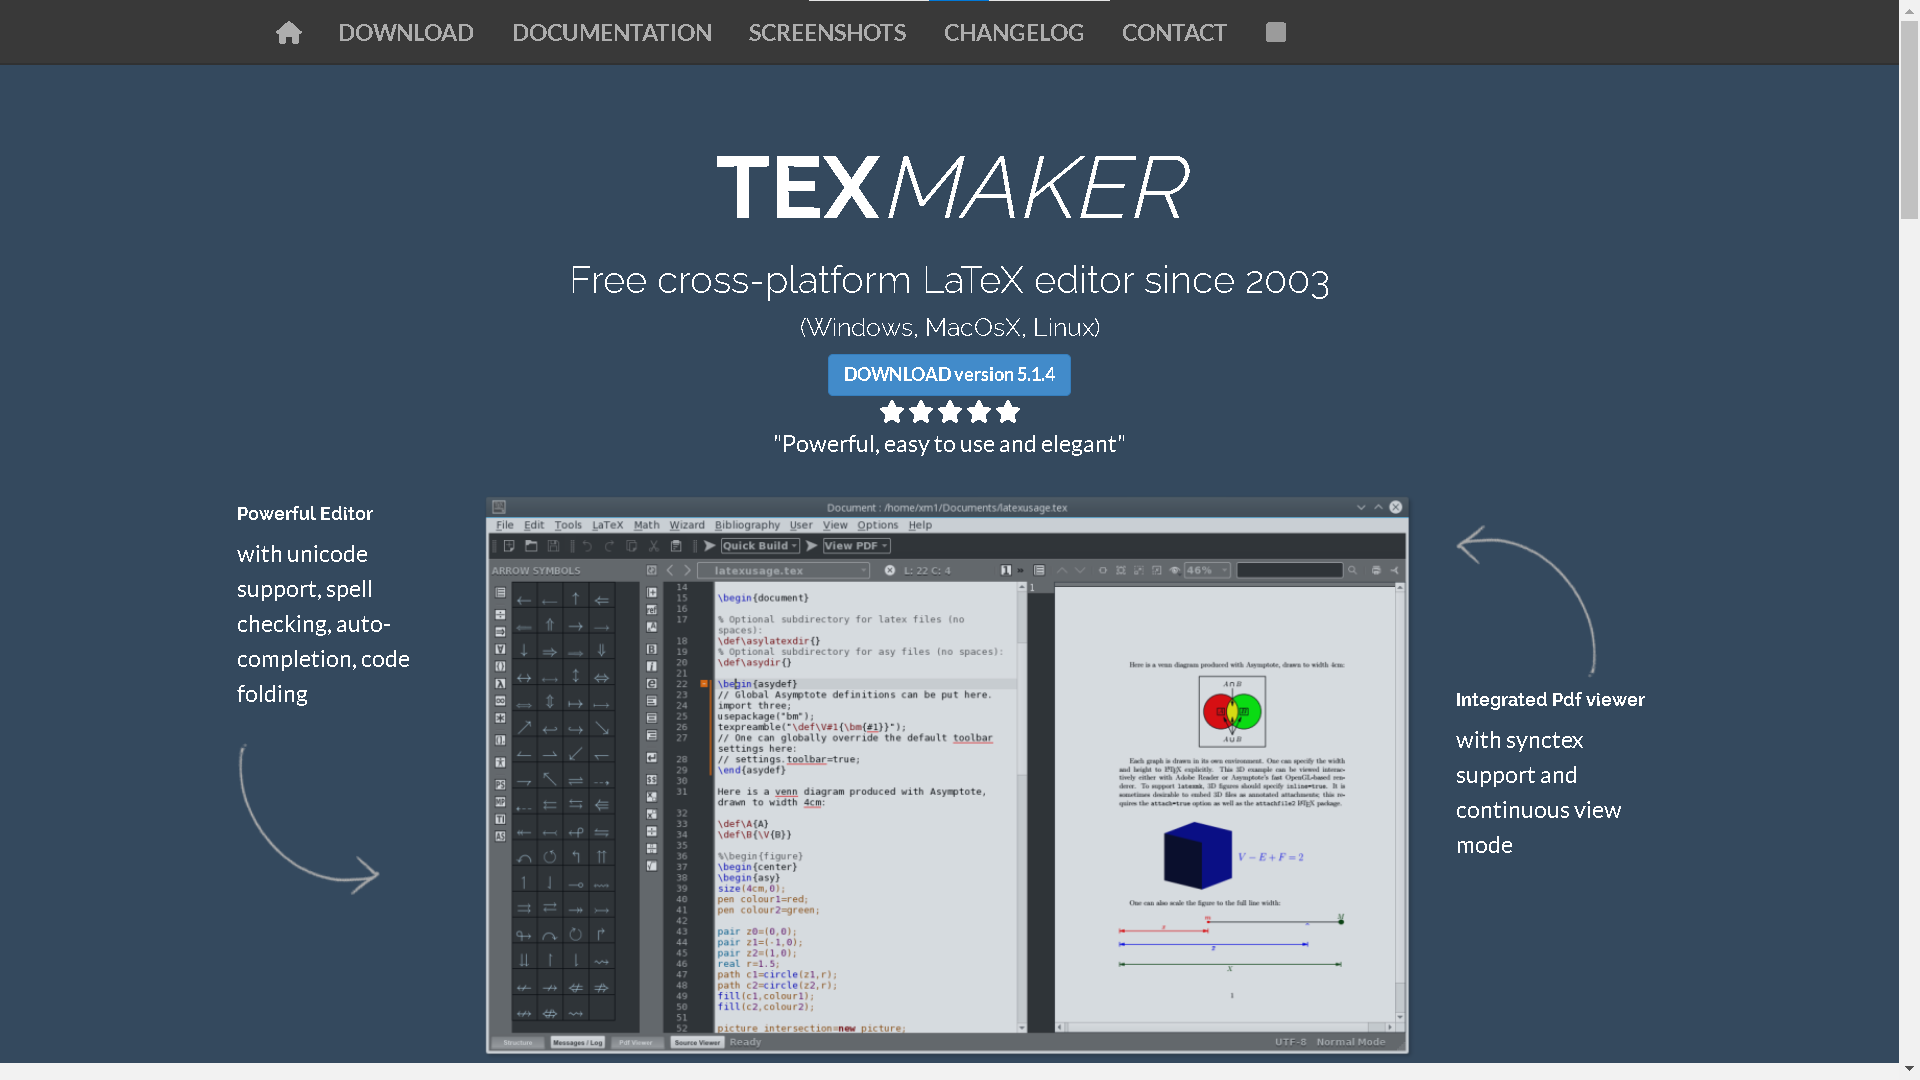
\includegraphics[width=1.0\linewidth,height=0.5\linewidth]{figure-0011.png}
  \caption{Начална уеб страница на Texmaker}
\label{figure-0011}
\end{figure}

Отново се избира тази версия за инсталиране, която е предназначена за използване под операционна система Windows (Фиг. \ref{figure-0012}).

\begin{figure}
  \centering
  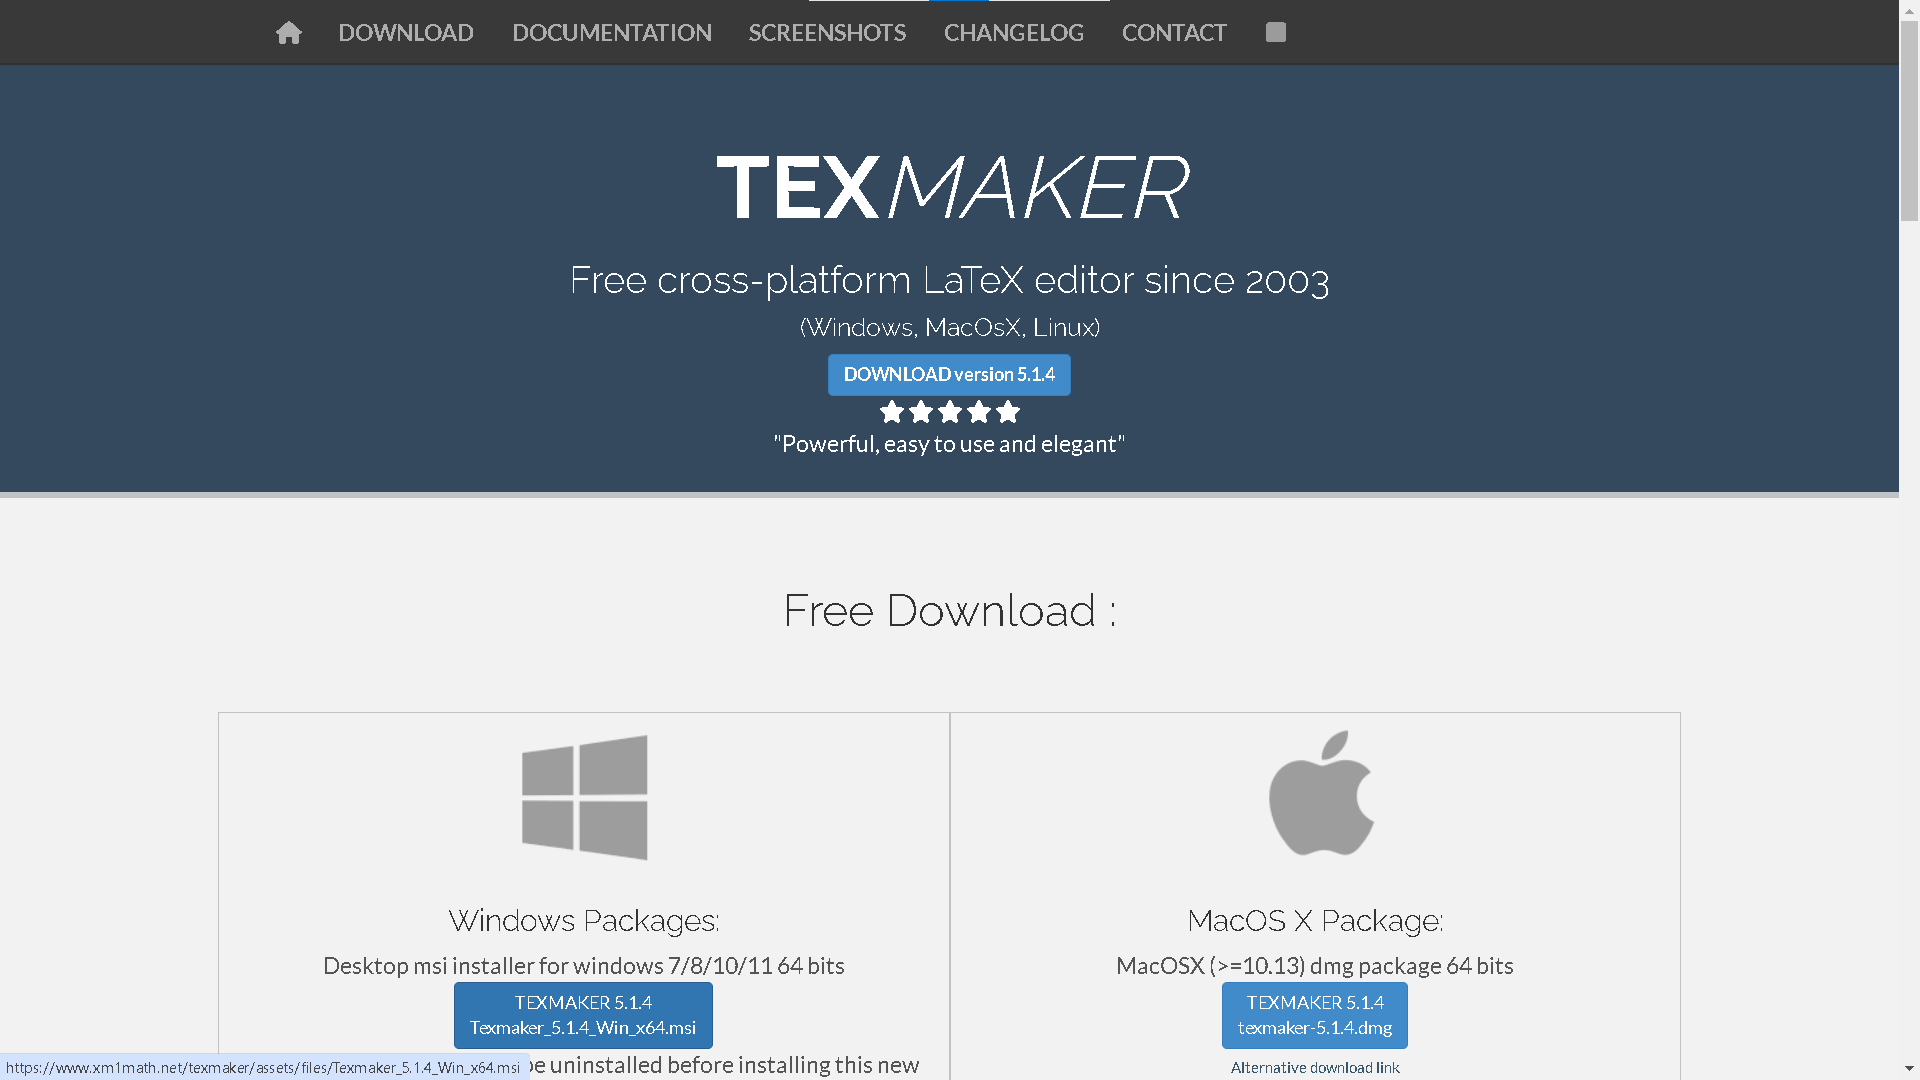
\includegraphics[width=1.0\linewidth,height=0.5\linewidth]{figure-0012.png}
  \caption{Избор на инсталационен файл за Texmaker}
\label{figure-0012}
\end{figure}

Потребителят бива информиран за юридическата рамка при която се съгласява да използва Texmaker, както и че за да бъде извършена инсталацията са необходими администраторски правомощия (Фиг. \ref{figure-0013}).

\begin{figure}
  \centering
  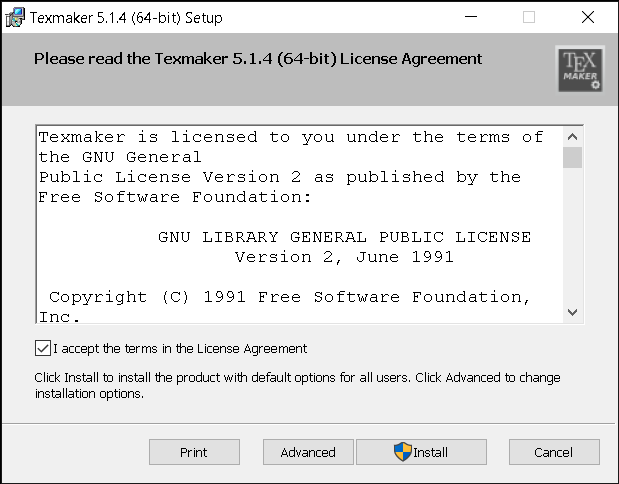
\includegraphics[width=1.0\linewidth,height=0.5\linewidth]{figure-0013.png}
  \caption{Диалогов прозорец за съгласие с условията за ползване на Texmaker}
\label{figure-0013}
\end{figure}

След приключване на процеса по инсталация, в диалогов прозорец се визуализира резултата и се дава възможност на потребителя да стартира програмата (Фиг. \ref{figure-0014}).

\begin{figure}
  \centering
  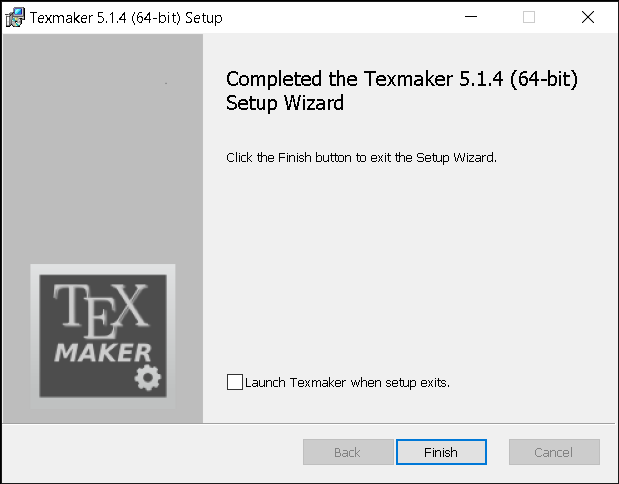
\includegraphics[width=1.0\linewidth,height=0.5\linewidth]{figure-0014.png}
  \caption{Диалогов прозорец с информация за извършеното инсталиране}
\label{figure-0014}
\end{figure}

Макар и успешно инсталирани, дали двата софтуера работят коректно най-добре може да се потвърди с изпълнението на минималистичен пример за LaTeX документ.

\section{Първоначален пример}

Направата на примерен документ започва със създаването на нов файл в работното пространство на Texmaker (Фиг. \ref{figure-0015}).

\begin{figure}
  \centering
  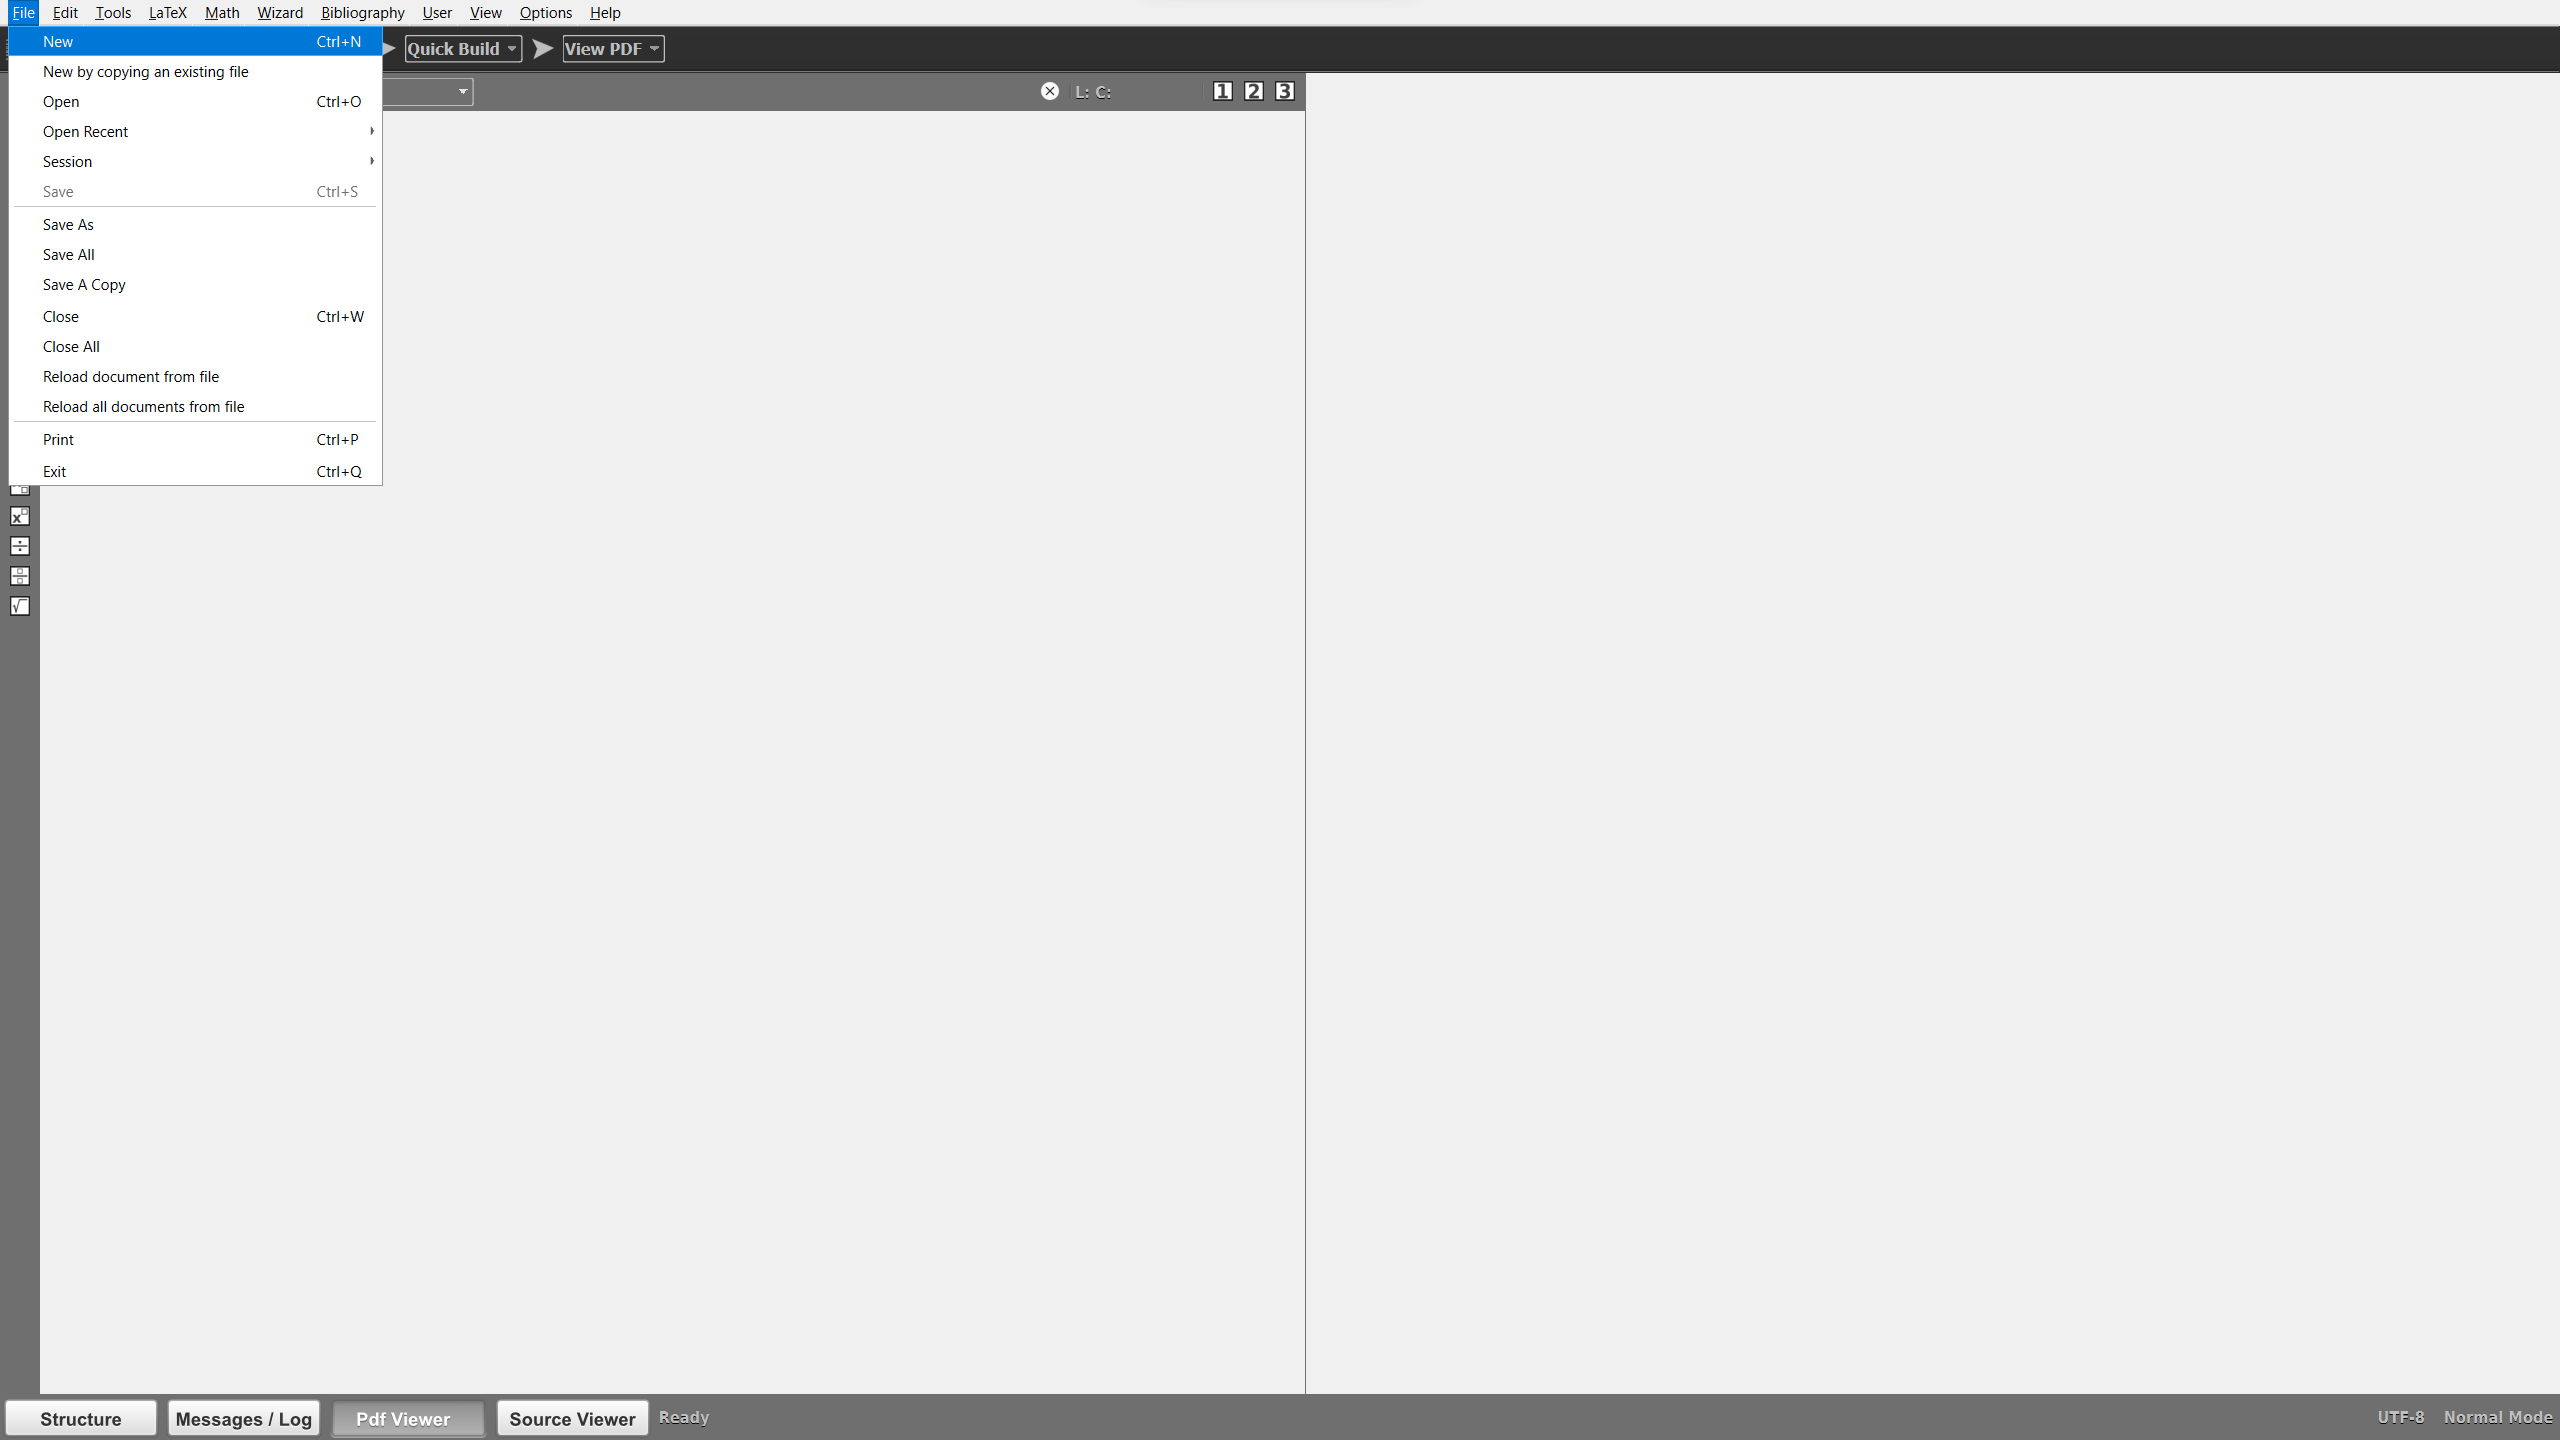
\includegraphics[width=1.0\linewidth,height=0.5\linewidth]{figure-0015.png}
  \caption{Създаване на нов документ в Texmaker}
\label{figure-0015}
\end{figure}

Следва въвеждане на минималния набор от команди, които водят до оформянето на завършен LaTeX документ (Лист. \ref{listing-0001}).

\begin{lstlisting}[language={[LaTeX]TeX}, caption=Минимален шаблон за LaTeX документ, label=listing-0001]
\documentclass{article}
\begin{document}

A journey of a thousand miles begins with a single step.

\end{document}

\end{lstlisting}

В демонстрирания пример се използва предварително дефиниран клас за описване на статия. Следва команда за начало на документа, текстово изложение и край на документа.

След запазване на документа, под името example-0001.tex, следва компилация (Tools -> Quick Build) и  визуализация на крайния резултат (Фиг. \ref{figure-0016}).

\begin{figure}
  \centering
  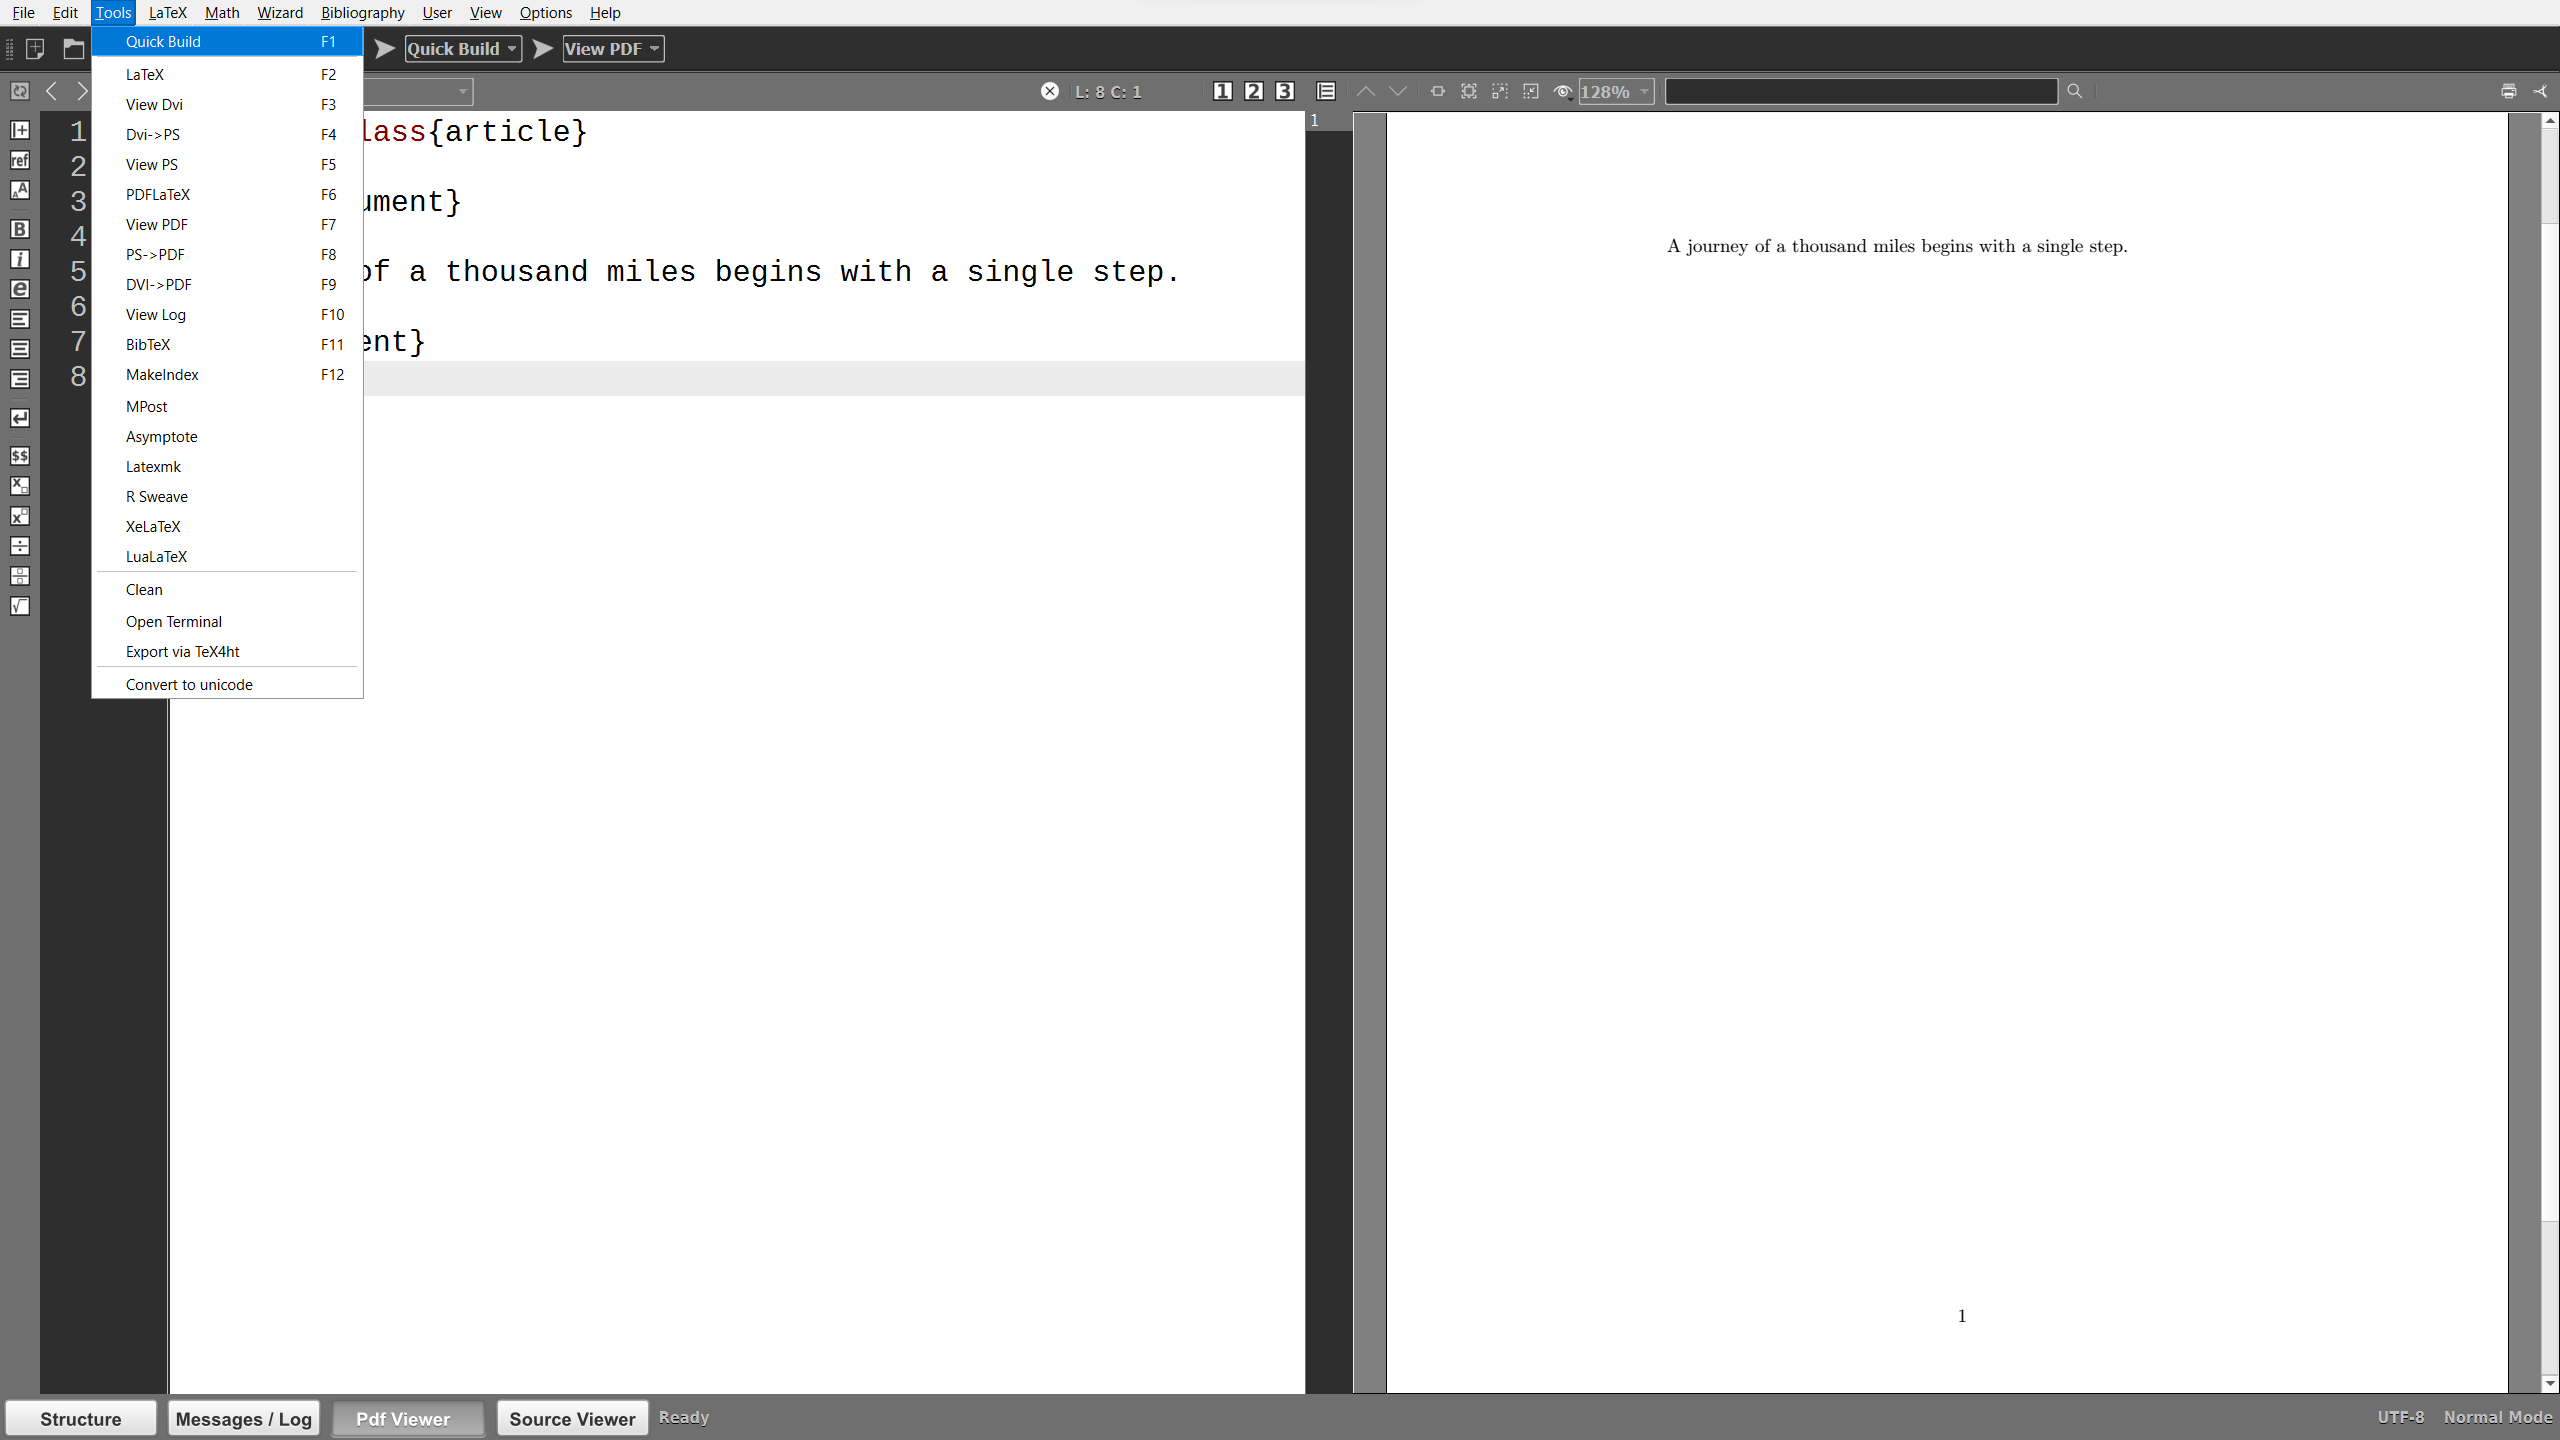
\includegraphics[width=1.0\linewidth,height=0.5\linewidth]{figure-0016.png}
  \caption{Компилиране на първоначален документ}
\label{figure-0016}
\end{figure}

За разлика от масово разпространените софтуерни инструменти за текстообработка, при LaTeX резултатът се получава след компилация, а не моментално в процеса на писане.

\section*{Обощение}

Като първи стъпи бяха свалени нужните софтуерни продукти, бяха инсталирани и настроение. С демонстрацията на базов, първоначален пример се демонстрира правилното функциониране на софтуерните инструменти.



\chapter{Форматиране на текст}
След успешното създаване на първоначален документ, може да се пристъпи към по-сериозно оформление на текста и детайлите около него. Ще бъде разяснено логическото форматиране, как LaTeX чете входната информация, как да се модифицират шрифтовете, оформление на полета, параграфи, подравняване и цитиране.

\section{Логическо форматиране}

В самият текст на LaTeX документа не се изпълнява физическо форматиране. Авторът не се грижи дали текстът е нормален, удебелен, наклонен, подчертан или нещо друго. За целите на оформлението се използва логическо форматиране. Документът има различни фрагменти, като заглавие, име на автор, секция, подсекция и други. Физическото форматиране се извършва от LaTeX според вида на компонента и предварително заредения шаблон. 

В много редки случаи, когато става въпрос за единични изключения е допустимо да се използва и физическо форматиране, но то значително затруднява последващата поддръжка на единно оформление в документа.

Добре оформеният LaTeX документ използва физическо форматиране само в командите, които указват изпълнението на физическото форматиране.

С един много опростен документ се демонстрират най-съществените части от оформлението, като: заглавие, автор, дата и основен текст.

\begin{lstlisting}[language={[LaTeX]TeX}, caption=Инструкция за вида на документа, label=listing-0002]
\documentclass[a4paper,11pt]{article}
\end{lstlisting}

Спрямо вида на документа (Лист. \ref{listing-0002}), LaTeX зарежда необходимите инструкции и стилово оформление. В първата инструкция се задава на носителя на информация (хартия формат А4) и размера на основния текст. 

\begin{lstlisting}[language={[LaTeX]TeX}, caption={Добавяне на заглавие, автор и дата}, label=listing-0003]
\documentclass[a4paper,11pt]{article}

\title{The Story of My Life}

\author{Dessislava Gruncharova}

\date{April 21, 1979}
\end{lstlisting}

Най-съществените атрибути на един документ са заглавието, автора и дата на създаване. За всяко от трите има подходящо дефинирана инструкция (Лист. \ref{listing-0003}).

\begin{lstlisting}[language={[LaTeX]TeX}, caption=Тяло на документа, label=listing-0004]
\documentclass[a4paper,11pt]{article}

\title{The Story of My Life}

\author{Dessislava Gruncharova}

\date{April 21, 1979}

\begin{document}
\end{document}
\end{lstlisting}

След описателната част на документа следва основното изложение (Лист. \ref{listing-0004}).

\begin{lstlisting}[language={[LaTeX]TeX}, caption=Инструкция за създаване на заглавна страница, label=listing-0005]
\documentclass[a4paper,11pt]{article}

\title{The Story of My Life}

\author{Dessislava Gruncharova}

\date{April 21, 1979}

\begin{document}

\maketitle

\end{document}
\end{lstlisting}

Заглавната страница се съставя автоматично с помощта на командата maketitle (Лист. \ref{listing-0005}).

\begin{lstlisting}[language={[LaTeX]TeX}, caption=Оформяне на секция в документа, label=listing-0006]
\documentclass[a4paper,11pt]{article}

\title{The Story of My Life}

\author{Dessislava Gruncharova}

\date{April 21, 1979}

\begin{document}

\maketitle

\section{The beginning was ...}

\end{document}
\end{lstlisting}

В LaTeX възприетият принцип е документът да се разделя на секции (Лист. \ref{listing-0006}).

\begin{lstlisting}[language={[LaTeX]TeX}, caption=Текстово изложение, label=listing-0007]
\documentclass[a4paper,11pt]{article}

\title{The Story of My Life}

\author{Dessislava Gruncharova}

\date{April 21, 1979}

\begin{document}

\maketitle

\section{The beginning was ...}

The story of my life started ...

\end{document}
\end{lstlisting}

След което следва същинското текстово изложение (Лист. \ref{listing-0007}).

\begin{figure}
  \centering
  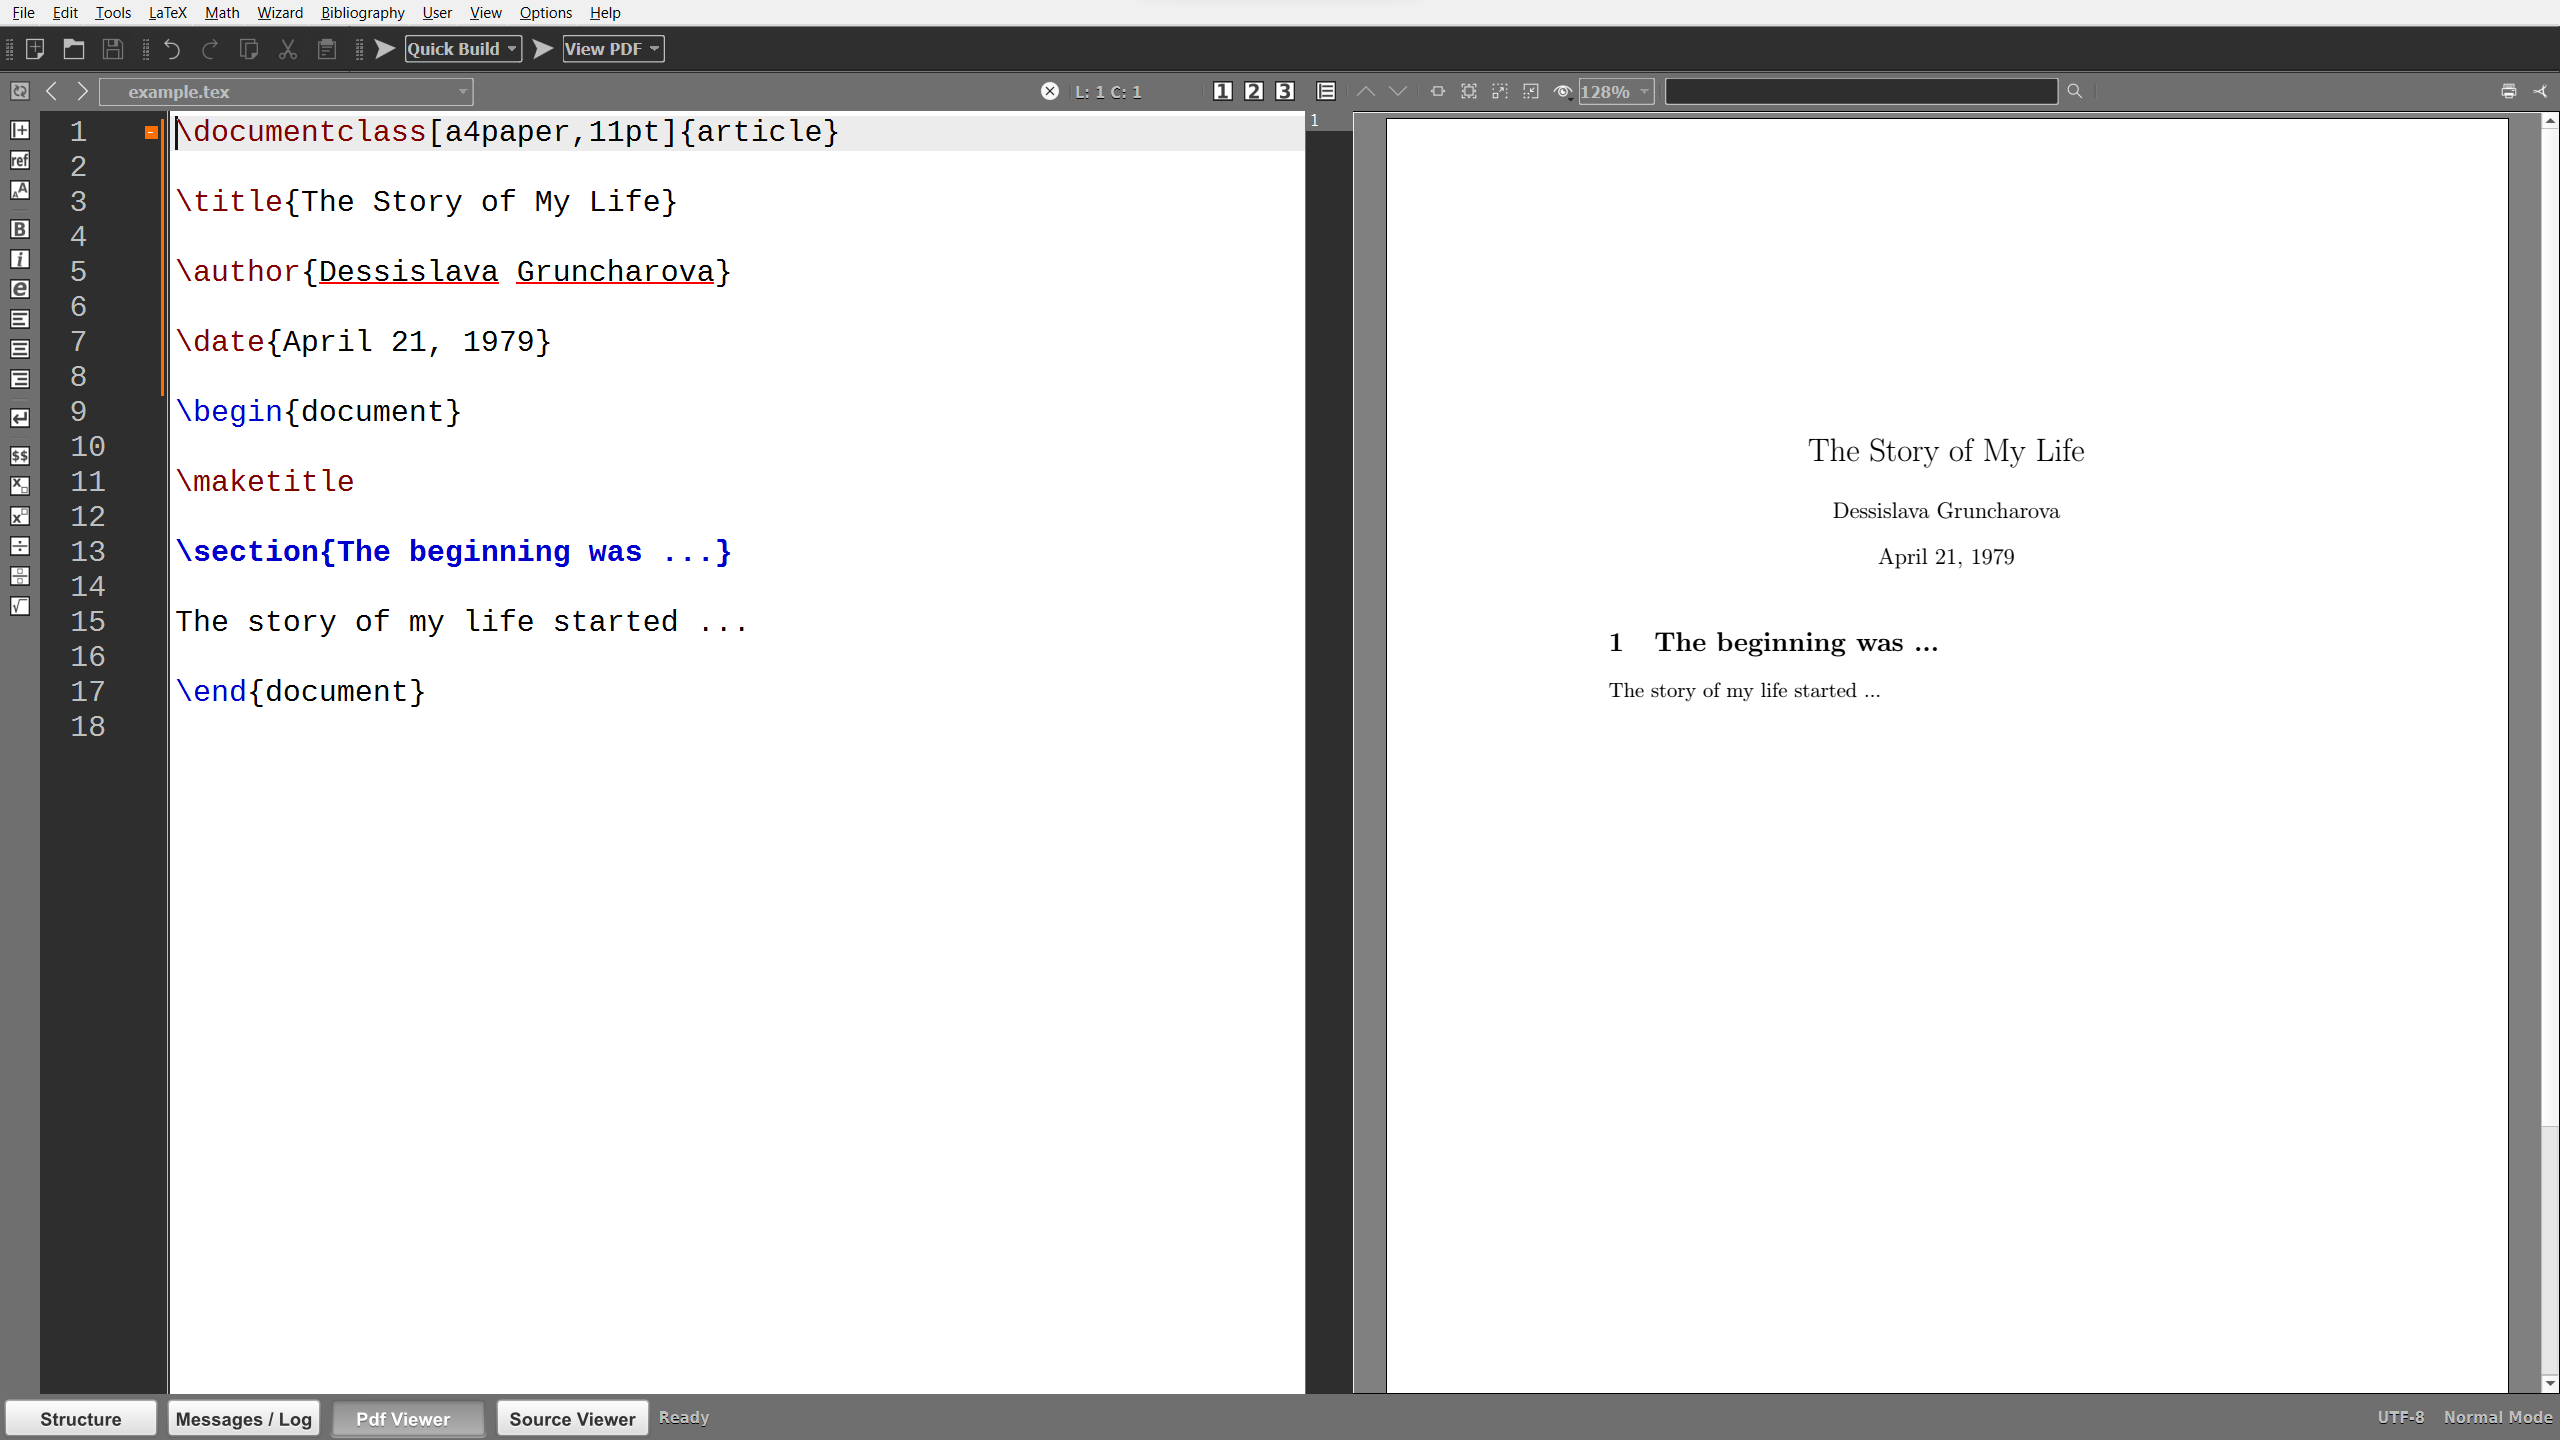
\includegraphics[width=1.0\linewidth,height=0.5\linewidth]{figure-0017.png}
  \caption{Резултат от компилацията с LaTeX}
\label{figure-0017}
\end{figure}

В резултат на извършената компилация, Texmaker предлага финалният PDF документ (Фиг. \ref{figure-0017}). Както може да се забележи, никъде не се указва размера на шрифта или графичното оформление за заглавието, автора и датата на публикуване. Всичко това е дефинирано в шаблона article. 

Важно е да се отбележи, че инструкциите в LaTeX основно започват с обратна наклонена черата, която е последвана от малки и големи букви. В повечето случай названията на инструкциите са самообясняващи се. Параметри на инструкциите се задават в къдрави скоби. Не задължителните параметри се ограждат в квадратни скоби. Освен инструкции в LaTeX има и фрагменти. Всеки фрагмент започва с ключова дума begin и завършва с ключова дума end. Както при командите, в къдрави скоби са задължителните аргументи, а в квадратни скоби са не задължителните аргументи. Във фрагмент се поставят, примерно, изображенията, листингите, таблиците и много други. 

\section{Обработка на входящата информация}

Тъй като LaTeX използва синтаксис от групата на тагиращите езици, то потокът от празни интервали и празни редове се управлява с команди. Дори да бъдат въведени множество символи за празен интервал, те се интепретират за един. Същата логика се прилага и за символът нов ред. Първият символ за нов ред обозначава началото на нов параграф, а всеки следващ символ за нов ред се игнорира в резултатния PDF документ. 

В процеса на тагиране често се налага частично да се изключват определени команди. Това може да се постигне с използването на коментари. Символът процент, в контекста на LaTeX документ, има смисъл на едноредов коментар. Също така, много добра практика е да се пишат коментари около по-значимите LaTeX команди. Обикновено коментарите са съпровождаща информация, която подпомага други автори на документа или самият автор, който се връща към този документ след определен период от време. 

В общия случай, текстовите документи се състоят предимно от букви, цифри и пунктуация, но понякога се налага използването на по-малко популярни символи. Налага се и използването на символът процент. Тъй като процентът има своя собствена интерпретация, то появата му в текста създаван от автора би довело до нежелана ситуация на LaTeX коментиране. За да се позволи използването на специални символи и символи имащи специфична интерпретация от езиковия процесор се прилага допълнително тагиране. Символът за обратна наклонена черта влиза в ролята на escape symbol. Това означава, че обърнатата наклонена черта предхожда специалния символ, така че да предизвика визуализацията на самия специален символ в текстовото изложение. Също така, налични са множество специално заделени тагове, включването на които водят до изписване на специални символи. 

\section{Боравене с шрифтове}

В относително редки случаи се налага да се акцентира върху думи или фрази в текста, когато не е удачно да се използва логическо форматиране. Такъв акцент може да се постигне с наклонен шрифт, удебелен шрифт, подчертаване на думи или някаква друга форма на декорация. В LaTeX са достъпни серия команди за локално оформление на текста, които могат да се вграждат една в друга (Лист. \ref{listing-0008}). Командите следват формата \textbackslash text**, където двете звездички се заменят с двубуквено съчетание. Като пример \textbackslash textbf (удебеляване) или \textbackslash textit (накланяне). Многократното влагане на една от тези команди, сама в себе си, не води до включване и изключване на характеристиката. Това не важи за командата \textbackslash emph. При рекурсивно влагане, тази команда преминава от нормален текст в наклонен и обратното. 

\begin{lstlisting}[language={[LaTeX]TeX}, caption=Вложено оформление, label=listing-0008]
\documentclass[a4paper,11pt]{article}

\title{The Story of My Life}

\author{Dessislava Gruncharova}

\date{April 21, 1979}

\begin{document}

\maketitle

\section{The beginning was ...}

The \textit{story of \textbf{my} life} started ...

\end{document}
\end{lstlisting}

По отношение на широко използваните шрифтове има една основна характеристика, която ги разделя и това е широчината на всяка отделна буква. Кондензираните шрифтове са тези при които по-тесните букви се изобразяват на по-късо разстояние, а по-широките букви се изобразяват на по-дълго разстояние. Този вид представяне на буквите преследва две цели, а именно ергономия на четене и оптимално използване на хартиения носител. Вторият тип шрифтове са моноспейсните шрифтове или шрифтовете за пишещи машини. Характерно за тях е, че всяка буква е изобразена с еднаква ширина. За преминаването към такъв шрифт, LaTeX предлага командата \textbackslash texttt. 

Второ разделение сред масово използваните шрифтове е според това дали буквите имат серифи или нямат. Когато буквите имат малки чертички по ръбчетата си (серифи) това е категорията на серифните шрифтове или на романските шрифтове. Романските шрифтове се използват основно при декоративни надписи, които трябва да привлекат вниманието на наблюдателя. Романските шрифтове затрудняват ергономията на четене и е желателно а се избягват при създаването на дълги текстове. Обратно на романските шрифтове са шрифтовет без серифи. При тези шрифотве буквите нямат добавени чертички, а понякога самите ръбове на буквите са заоблени. В LaTeX, преминаването към несерифен шрифт може постигне с командата \textbackslash textsf. 

За по-големи пасажи текст, LaTeX предлага превключване на шрифтовете. 

\section{Оформяне на зони и параграфи}



\section{Подравняване и цитиране}



\section*{Обобщение}





\part{Част II}

\chapter{Глава 3}

\chapter{Глава 4}

\part{Част III}

\chapter{Глава 5}

\chapter{Глава 6}

\appendix

\chapter{Приложение 1}

\backmatter

\chapter{Библиография}
\begin{thebibliography}{99}
\end{thebibliography}


\end{document}
